% =============================================================================
%  SECTION 5 --- BEAMER SLIDE DECK
%  "How Close Are We to AGI? A Reality Check for Decision-Makers"
%  ETH Zurich Executive Education --- 90-minute lecture
% =============================================================================
\documentclass[aspectratio=169, 12pt, xcolor={dvipsnames,table}]{beamer}

% --- Theme ------------------------------------------------------------------
\usetheme{metropolis}
\setbeamercolor{normal text}{fg=black!85, bg=white}
\setbeamercolor{alerted text}{fg=BrickRed}
\setbeamercolor{frametitle}{bg=black!85, fg=white}
\setbeamertemplate{navigation symbols}{}
\setbeamerfont{title}{size=\Large, series=\bfseries}
\setbeamerfont{frametitle}{size=\large, series=\bfseries}
\setbeamerfont{footnote}{size=\tiny}

% --- Packages ---------------------------------------------------------------
\usepackage[T1]{fontenc}
\usepackage{lmodern}
\usepackage{amsmath, amssymb}
\usepackage{tikz}
\usetikzlibrary{arrows.meta, positioning, calc, fit, backgrounds, matrix, shapes.geometric}
\usepackage{pgfplots}
\pgfplotsset{compat=1.18}
\usepackage{booktabs}
\usepackage{appendixnumberbeamer}
\usepackage[round]{natbib}

% --- Macros -----------------------------------------------------------------
\newcommand{\bigquote}[1]{%
  \begin{center}
    \large\itshape ``#1''
  \end{center}
}
\newcommand{\sourcemark}[1]{\hfill{\tiny\color{gray}#1}}

% --- Metadata ---------------------------------------------------------------
\title{How Close Are We to AGI?}
\subtitle{A Reality Check for Decision-Makers}
\author{ETH Zurich Executive Education}
\date{2026}
\institute{}

% ============================================================================
\begin{document}

% --- 1. TITLE ---------------------------------------------------------------
\begin{frame}[plain]
  \vspace*{-2em}
  \titlepage
\end{frame}

% --- 2. SESSION OVERVIEW ----------------------------------------------------
\begin{frame}{Session Overview --- Five Acts in Ninety Minutes}
\vspace{0.3em}
\renewcommand{\arraystretch}{1.35}
\begin{center}
\begin{tabular}{@{}p{1.2cm} p{7.5cm} p{4.8cm}@{}}
\toprule
\textbf{Act} & \textbf{Theme} & \textbf{Anchor reference}\\
\midrule
\rowcolor{NavyBlue!10}    1 & What IS AGI? & Morris et al., ICML 2024\\
\rowcolor{NavyBlue!15}    2 & Sparks \& Specialist Breakthroughs & Bubeck 2023; \emph{Nature} 2024\\
\rowcolor{BrickRed!10}    3 & Chatbots to Agents & METR, 2024--2026\\
\rowcolor{BrickRed!15}    4 & When Will AGI Arrive? & Grace et al.\ 2024, $N{=}2778$\\
\rowcolor{ForestGreen!15} 5 & Managing the Transition & Bengio--Hinton--Russell, \emph{Science} 2024\\
\bottomrule
\end{tabular}
\end{center}
\note{Signpost the arc. Emphasise that each act is built around one anchor
reference, and that the session's job is to put that reference in their
hands calibrated, not to tell them when AGI arrives.}
\end{frame}

% ============================================================================
% ACT 1
% ============================================================================
\section{Act 1 --- What IS AGI?}

\begin{frame}[plain]
\begin{center}
  {\Huge\bfseries Act 1}\\[0.4em]
  {\large What Do We Mean by AGI?}\\[1.5em]
  {\footnotesize\itshape Anchor: Morris et al., ``Levels of AGI,'' ICML 2024}
\end{center}
\note{Pause. Promise they will leave the act with a shared vocabulary, not
a timeline.}
\end{frame}

\begin{frame}{The Question Everyone Is Asking}
\bigquote{Is this thing actually intelligent --- or just very good at
autocomplete?}
\vspace{1em}
\begin{itemize}
  \item The phrase ``AGI'' is now in press releases, contracts, and regulation.
  \item Five years ago, serious researchers avoided it in public.
  \item \textbf{If the term is fuzzy, the obligation is fuzzy.}
\end{itemize}
\note{Open with the board-member framing: this is a contractual and regulatory
question, not just a philosophical one.}
\end{frame}

\begin{frame}{The Morris et al.\ Framework --- Two Axes}
\begin{center}
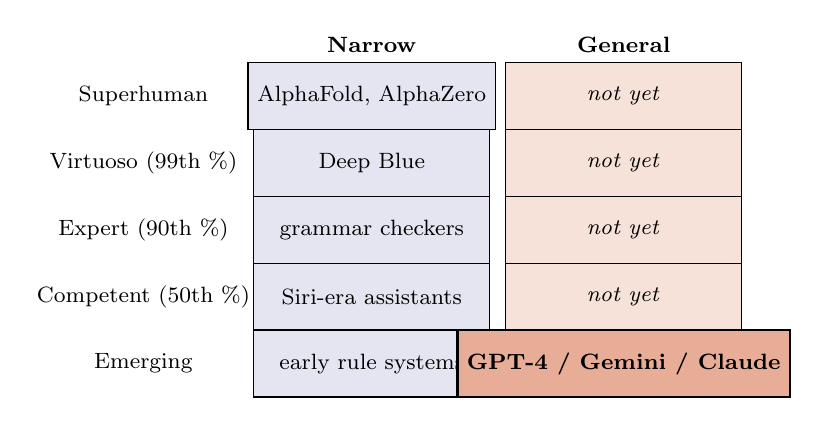
\begin{tikzpicture}[font=\footnotesize,
  cell/.style={draw, minimum width=3.0cm, minimum height=0.85cm, align=center},
  row/.style={draw=none, minimum width=2.8cm, align=right},
  col/.style={draw=none, align=center}]

  % Column headers
  \node[col] at (1.8,3.2) {\bfseries Narrow};
  \node[col] at (5.0,3.2) {\bfseries General};

  % Row headers (performance)
  \node[row] at (-1.1, 2.55) {Superhuman};
  \node[row] at (-1.1, 1.70) {Virtuoso (99th \%)};
  \node[row] at (-1.1, 0.85) {Expert (90th \%)};
  \node[row] at (-1.1, 0.00) {Competent (50th \%)};
  \node[row] at (-1.1,-0.85) {Emerging};

  % Cells (narrow)
  \node[cell, fill=NavyBlue!10] at (1.8, 2.55) {AlphaFold, AlphaZero};
  \node[cell, fill=NavyBlue!10] at (1.8, 1.70) {Deep Blue};
  \node[cell, fill=NavyBlue!10] at (1.8, 0.85) {grammar checkers};
  \node[cell, fill=NavyBlue!10] at (1.8, 0.00) {Siri-era assistants};
  \node[cell, fill=NavyBlue!10] at (1.8,-0.85) {early rule systems};

  % Cells (general)
  \node[cell, fill=BrickRed!10] at (5.0, 2.55) {\textit{not yet}};
  \node[cell, fill=BrickRed!10] at (5.0, 1.70) {\textit{not yet}};
  \node[cell, fill=BrickRed!10] at (5.0, 0.85) {\textit{not yet}};
  \node[cell, fill=BrickRed!10] at (5.0, 0.00) {\textit{not yet}};
  \node[cell, fill=BrickRed!30, thick] at (5.0,-0.85) {\textbf{GPT-4 / Gemini / Claude}};

\end{tikzpicture}
\end{center}
\vspace{0.3em}
{\tiny Adapted from \citet{morris2024levels}.}
\note{This is the slide to linger on. Point to the bottom-right cell. DeepMind's
own framework says today's frontier models are only ``Emerging'' on generality.
Everything above it --- Competent, Expert, Virtuoso, Superhuman --- on the
general column, is empty.}
\end{frame}

\begin{frame}{Where Frontier Models Sit Today}
\bigquote{Emerging General AGI.}
\begin{itemize}
  \item \textbf{More than} the public sometimes hears: a genuinely new category of artefact.
  \item \textbf{Less than} the marketing sometimes claims: not yet \emph{competent} across domains.
  \item \textbf{No press release} will announce AGI. You will notice it workflow by workflow.
\end{itemize}
\note{Resist the temptation to debate whether this is the ``right'' level.
The point is that we now have a \emph{shared axis} to argue on.}
\end{frame}

\begin{frame}{Counterweight: Chollet's ``Measure of Intelligence''}
\begin{center}
\itshape Intelligence is the \textbf{efficiency} with which a system\\ acquires new skills
in a previously unseen domain,\\ using limited prior knowledge and limited experience.
\end{center}
\vspace{0.6em}
\begin{itemize}
  \item Benchmark scores can reflect \emph{memorisation + interpolation}.
  \item ARC-AGI: designed to resist training-data overlap.
  \item Was only substantially cracked in late 2024 --- and at high compute cost.
\end{itemize}
\sourcemark{\citealp{chollet2019measure}}
\note{The honest read: use Morris to locate systems, use Chollet to stress-test
whether the location is real. In procurement: require the vendor to evaluate
on held-out tasks \emph{you} pick.}
\end{frame}

\begin{frame}{Act 1 Takeaway}
\begin{itemize}
  \item We have a vocabulary: \textbf{performance $\times$ generality}.
  \item Today's frontier models: \textbf{Emerging General AGI}.
  \item When a vendor says ``approaching AGI,'' ask:\\
        \quad \emph{On which axis? Against what reference distribution?}
\end{itemize}
\note{Before moving on, restate the test they should now apply to any vendor
claim. If they remember only one slide from Act 1, this is the one.}
\end{frame}

% ============================================================================
% ACT 2
% ============================================================================
\section{Act 2 --- Sparks \& Specialist Breakthroughs}

\begin{frame}[plain]
\begin{center}
  {\Huge\bfseries Act 2}\\[0.4em]
  {\large What Can the Best Systems Already Do?}\\[1.5em]
  {\footnotesize\itshape Anchors: Bubeck et al., \emph{Sparks of AGI}, 2023;\\
   Trinh et al., AlphaGeometry, \emph{Nature} 2024}
\end{center}
\note{Two systems, two paradigms: a generalist with emerging abilities, and
a specialist that beats humans cold.}
\end{frame}

\begin{frame}{Bubeck et al., ``Sparks of AGI''}
\bigquote{We could reasonably view GPT-4 as an early (yet still
incomplete) version of an AGI system.}
\vspace{0.6em}
\begin{itemize}
  \item 155-page technical report, Microsoft Research, March 2023.
  \item Qualitative probes: maths, code, vision-via-TikZ, theory of mind, analogy.
  \item The \emph{claim} broke the taboo. The \emph{paper} is honest about its limits.
\end{itemize}
\sourcemark{\citealp{bubeck2023sparks}}
\note{The shock was not the evidence --- it was that senior researchers at
a major lab were willing to put the sentence above in print.}
\end{frame}

\begin{frame}{Sparks --- The Honest Caveats}
\begin{itemize}
  \item Tested an \textbf{early, pre-alignment} GPT-4 (no RLHF yet).
  \item \textbf{Could not inspect training data} --- contamination possible.
  \item Authors explicit about \textbf{cherry-picking interesting examples}.
  \item Schaeffer--Miranda--Koyejo (NeurIPS 2023, Outstanding Paper):
        ``emergence'' partly a \emph{measurement} artefact.
\end{itemize}
\sourcemark{\citealp{schaeffer2023mirage}}
\note{This is where a calibrated briefing earns trust. Acknowledge the caveats
\emph{before} the audience raises them.}
\end{frame}

\begin{frame}{AlphaGeometry --- The Problem}
\begin{itemize}
  \item IMO-level Euclidean geometry: \emph{creative} insight required.
  \item Typical trick: introduce an auxiliary point, line, or circle.
  \item After the trick: symbolic deduction finishes the proof.
  \item Human geometry proofs are \textbf{scarce and hard to formalise}.
\end{itemize}
\sourcemark{\citealp{trinh2024alphageometry}}
\note{Set up why this domain is a good test: clear verifier (is the proof
valid?), but genuine creativity required.}
\end{frame}

\begin{frame}{AlphaGeometry --- Neuro-Symbolic Architecture}
\begin{center}
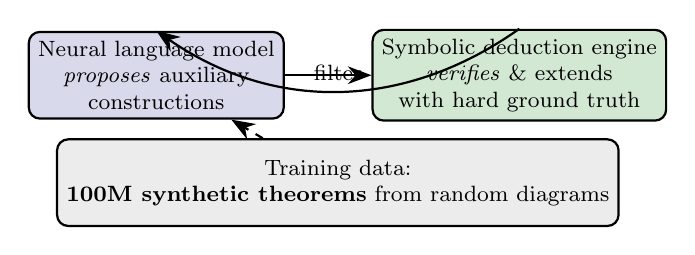
\begin{tikzpicture}[font=\footnotesize,
  node distance=0.8cm and 1.1cm,
  box/.style={draw, rounded corners, thick, minimum width=3.2cm,
              minimum height=1.1cm, align=center}]
  \node[box, fill=NavyBlue!15] (nn) {Neural language model\\ \emph{proposes} auxiliary\\ constructions};
  \node[box, fill=ForestGreen!20, right=of nn] (sym) {Symbolic deduction engine\\ \emph{verifies} \& extends\\ with hard ground truth};
  \node[box, fill=gray!15, below=of $(nn)!0.5!(sym)$] (data) {Training data:\\ \textbf{100M synthetic theorems} from random diagrams};

  \draw[-{Stealth[length=3mm]}, thick] (nn) -- (sym);
  \draw[-{Stealth[length=3mm]}, thick] (sym.north) to[bend left=35] node[above]{filter} (nn.north);
  \draw[-{Stealth[length=3mm]}, thick, dashed] (data) -- (nn);
\end{tikzpicture}
\end{center}
\vspace{0.4em}
\textbf{Zero human-written proofs in training.}
\note{The managerial point: wherever a domain has an automatic verifier, you
can generate your own training data. That pattern is not confined to geometry.}
\end{frame}

\begin{frame}{AlphaGeometry --- 25 out of 30 IMO Problems}
\begin{center}
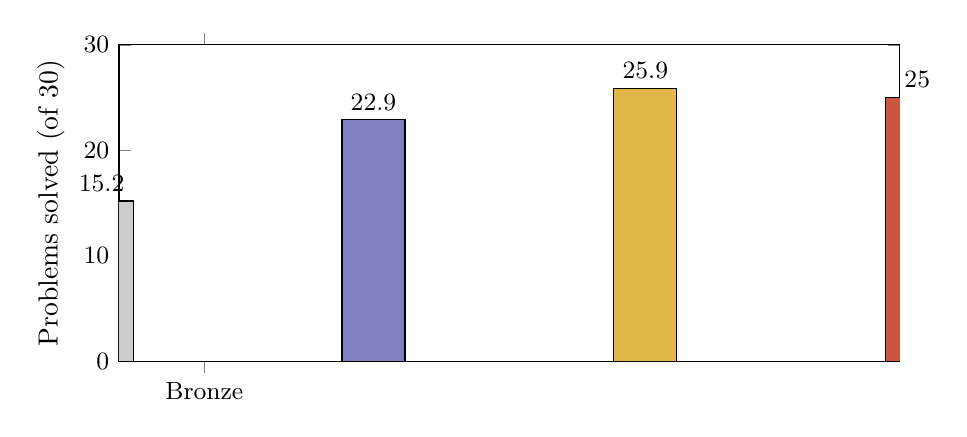
\begin{tikzpicture}
  \begin{axis}[
    width=11.5cm, height=5.6cm,
    ybar, bar width=0.8cm,
    enlarge x limits=0.14,
    ymin=0, ymax=30,
    ylabel={Problems solved (of 30)},
    symbolic x coords={Bronze, Silver, Gold, AlphaGeometry},
    xtick=data,
    nodes near coords,
    nodes near coords style={font=\small\bfseries},
    tick label style={font=\small},
  ]
    \addplot[fill=gray!40]       coordinates {(Bronze,15.2)};
    \addplot[fill=NavyBlue!50]   coordinates {(Silver,22.9)};
    \addplot[fill=Goldenrod!80]  coordinates {(Gold,25.9)};
    \addplot[fill=BrickRed!70]   coordinates {(AlphaGeometry,25)};
  \end{axis}
\end{tikzpicture}
\end{center}
\vspace{-0.3em}
{\footnotesize Human medallist averages vs.\ AlphaGeometry, 30 recent IMO
geometry problems.}
\note{AlphaProof + AlphaGeometry-2 (July 2024) then reached silver on the
full IMO --- algebra, combinatorics, number theory, geometry --- 28/42,
one below gold.}
\end{frame}

\begin{frame}{The Pattern That Matters for Managers}
\begin{center}
\bigquote{Domains with verifiers fall fast.\\ Domains without verifiers do not.}
\end{center}
\vspace{0.4em}
\begin{itemize}
  \item Verifier-rich: maths, code, games, formal compliance checks.
  \item Verifier-poor: taste, contested judgement, strategic persuasion.
  \item \textbf{Which parts of your business have a verifier --- or could?}
\end{itemize}
\note{This is the single most actionable frame from Act 2. Ask them to name,
in their heads, the nearest workflow in their org that has a machine-checkable
success criterion.}
\end{frame}

% ============================================================================
% ACT 3
% ============================================================================
\section{Act 3 --- From Chatbots to Agents}

\begin{frame}[plain]
\begin{center}
  {\Huge\bfseries Act 3}\\[0.4em]
  {\large From Chatbots to Agents: Measuring Autonomy}\\[1.5em]
  {\footnotesize\itshape Anchor: METR, ``Measuring AI Ability to Complete
   Long Tasks,'' 2024--2026}
\end{center}
\note{The shift from one-shot outputs to multi-stage trajectories is the most
important commercial development of the last two years.}
\end{frame}

\begin{frame}{What Is an ``Agent''?}
\begin{center}
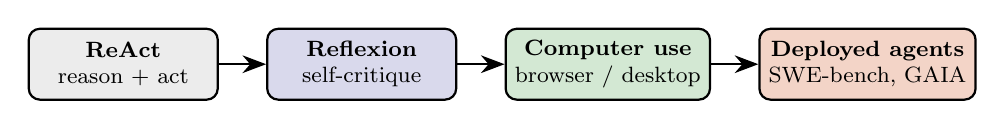
\begin{tikzpicture}[font=\footnotesize, node distance=0.5cm and 0.6cm,
  stage/.style={draw, rounded corners, thick, minimum width=2.4cm,
               minimum height=0.9cm, align=center}]
  \node[stage, fill=gray!15] (react)   {\textbf{ReAct}\\ reason + act};
  \node[stage, fill=NavyBlue!15, right=of react] (refl) {\textbf{Reflexion}\\ self-critique};
  \node[stage, fill=ForestGreen!20, right=of refl] (cu)  {\textbf{Computer use}\\ browser / desktop};
  \node[stage, fill=BrickRed!15, right=of cu]       (ag)  {\textbf{Deployed agents}\\ SWE-bench, GAIA};

  \draw[-{Stealth[length=3mm]}, thick] (react) -- (refl);
  \draw[-{Stealth[length=3mm]}, thick] (refl)  -- (cu);
  \draw[-{Stealth[length=3mm]}, thick] (cu)    -- (ag);
\end{tikzpicture}
\end{center}
\vspace{0.6em}
\textbf{Unit of work:} one-shot output $\longrightarrow$ multi-stage trajectory.\\[0.2em]
\textbf{Implication:} the right question becomes \emph{``for how long?''}
\sourcemark{\citealp{yao2023react}; \citealp{shinn2023reflexion}}
\note{Architectures matter less than the conceptual shift: AI is now evaluated
on trajectories, not answers.}
\end{frame}

\begin{frame}{METR --- The Task-Horizon Metric}
\begin{itemize}
  \item Portfolio of real engineering, research, data-analysis tasks.
  \item Measure \textbf{how long a skilled human needs} for each one.
  \item Ask: at what human-time horizon does the model succeed $\geq 50\%$ of the time?
  \item That number is the \textbf{50\% task horizon}.
\end{itemize}
\vspace{0.3em}
\textbf{Crucially:} third-party, not a vendor benchmark; rigorously
human-baselined; tracks a trend rather than saturating.
\sourcemark{\citealp{metr2024horizon}}
\note{Walk them through the definition slowly. This is the metric they should
internalise.}
\end{frame}

\begin{frame}{The METR Doubling Curve}
\begin{center}
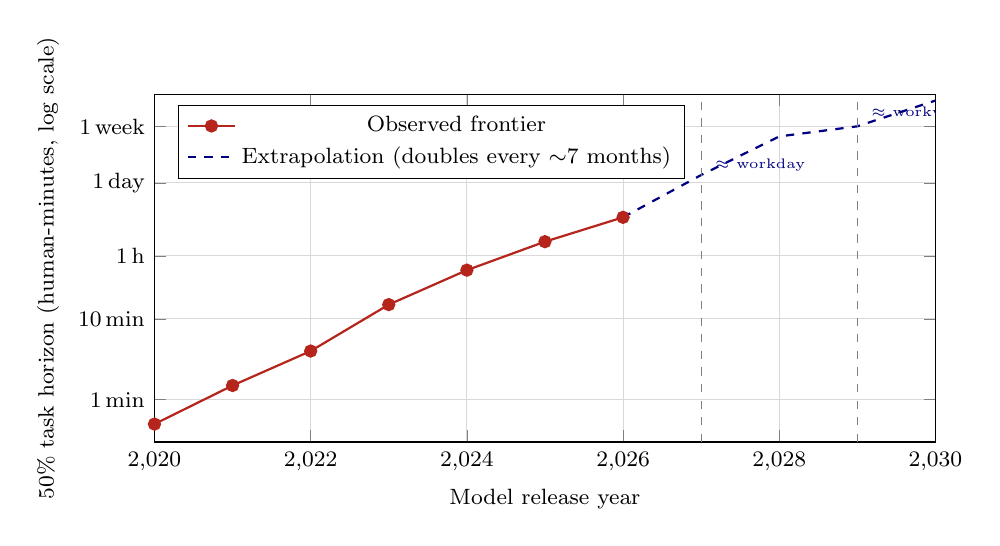
\begin{tikzpicture}
  \begin{semilogyaxis}[
    width=11.5cm, height=6.0cm,
    xlabel={Model release year},
    ylabel={50\% task horizon (human-minutes, log scale)},
    xmin=2020, xmax=2030,
    ymin=0.3, ymax=6000,
    xtick={2020,2022,2024,2026,2028,2030},
    ytick={1,10,60,480,2400},
    yticklabels={1\,min, 10\,min, 1\,h, 1\,day, 1\,week},
    grid=both,
    major grid style={gray!30},
    minor grid style={gray!10},
    legend pos=north west,
    legend style={font=\footnotesize},
    tick label style={font=\footnotesize},
    label style={font=\footnotesize},
  ]
    % doubling every ~7 months => factor 2^{12/7} per year ~ 3.28 per year
    \addplot[thick, BrickRed, mark=*, mark size=2pt]
      coordinates {(2020, 0.5)(2021, 1.5)(2022, 4)(2023, 15)(2024, 40)(2025, 90)(2026, 180)};
    \addlegendentry{Observed frontier}
    \addplot[thick, dashed, NavyBlue, no marks]
      coordinates {(2026, 180)(2027, 600)(2028, 1800)(2029, 2400)(2030, 5000)};
    \addlegendentry{Extrapolation (doubles every ${\sim}$7 months)}
    \draw[gray, dashed] (axis cs:2027,0.3) -- (axis cs:2027,6000);
    \draw[gray, dashed] (axis cs:2029,0.3) -- (axis cs:2029,6000);
    \node[NavyBlue, font=\tiny, anchor=south west] at (axis cs:2027.05, 500){$\approx$ workday};
    \node[NavyBlue, font=\tiny, anchor=south west] at (axis cs:2029.05, 2400){$\approx$ workweek};
  \end{semilogyaxis}
\end{tikzpicture}
\end{center}
\sourcemark{METR technical reports, 2024--2026. Values illustrative.}
\note{If the doubling holds at ~7 months, one working day arrives around 2027,
one working week around 2029. Big ``if''.}
\end{frame}

\begin{frame}{Extrapolation Is a Claim, Not a Measurement}
\textbf{Reasons the curve could bend down:}
\begin{itemize}
  \item Compute cost; energy and chip constraints.
  \item Data exhaustion for next-token pre-training.
  \item Long-horizon reliability is \emph{engineering}, not just scaling.
  \item A capability ceiling we do not yet understand.
\end{itemize}
\vspace{0.3em}
\textbf{Reasons it could accelerate:}
\begin{itemize}
  \item Reasoning models; better post-training; tool use; multi-agent systems.
\end{itemize}
\vspace{0.3em}
\alert{Track the curve quarterly. Re-plan when it bends.}
\note{Resist being a prophet. Be a good Bayesian. The curve is a leading
indicator, not a forecast with confidence intervals.}
\end{frame}

\begin{frame}{Supporting Evidence --- Same Shape, Different Axes}
\begin{itemize}
  \item \textbf{SWE-bench} \citep{jimenez2024swebench} --- real GitHub issues.
        From unusable to $>50\%$ on Verified variants.
  \item \textbf{GAIA} \citep{mialon2024gaia} --- general assistant tasks.
        Humans $\sim\!92\%$; frontier systems from $<15\%$ to $>50\%$ in 2.5 years.
  \item Both are contamination-resistant by construction.
  \item Both trace the same curve as the METR horizon.
\end{itemize}
\note{Converging evidence is the strong signal. Any one benchmark can be gamed
or contaminated; three independent ones moving together is harder to explain away.}
\end{frame}

% ============================================================================
% ACT 4
% ============================================================================
\section{Act 4 --- When Will AGI Arrive?}

\begin{frame}[plain]
\begin{center}
  {\Huge\bfseries Act 4}\\[0.4em]
  {\large When Will AGI Arrive?}\\[1.5em]
  {\footnotesize\itshape Anchor: Grace et al., \emph{Thousands of AI Authors
   on the Future of AI}, 2024}
\end{center}
\note{The act is less about the number 2047 and more about what the shape
of expert disagreement teaches you.}
\end{frame}

\begin{frame}{The Largest Expert Survey Ever Conducted}
\begin{itemize}
  \item \textbf{2,778 researchers} who published at NeurIPS / ICML.
  \item Survey run January 2023; prior run in 2022.
  \item Asks: when will \emph{High-Level Machine Intelligence} (HLMI) ---
        machines better and cheaper than humans at every task --- arrive?
  \item Also: specific-capability timelines, and probabilities of
        extreme outcomes.
\end{itemize}
\sourcemark{\citealp{grace2024thousands}}
\note{Emphasise: this is the people who build these systems rating their
own field. Not journalists. Not forecasters. Practitioners.}
\end{frame}

\begin{frame}{The 13-Year Shift}
\begin{center}
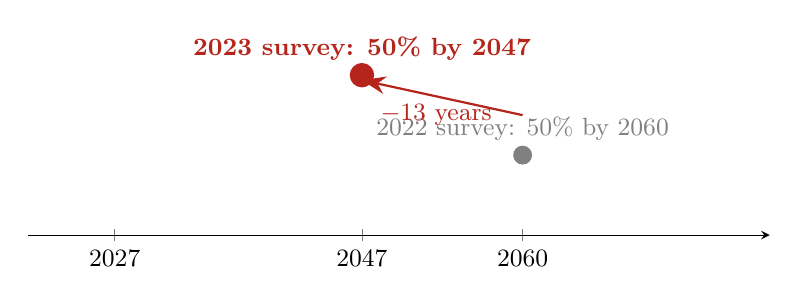
\begin{tikzpicture}
  \begin{axis}[
    width=11cm, height=4.5cm,
    xmin=2020, xmax=2080,
    ymin=0, ymax=2.3,
    ytick=\empty,
    xtick={2027,2047,2060,2100},
    xticklabels={2027, 2047, 2060, 2100},
    axis x line=bottom,
    axis y line=none,
    tick label style={font=\small},
  ]
    % 2022 survey: 50% in 2060
    \addplot[thick, gray, mark=*, mark size=3pt]
      coordinates {(2060, 0.8)};
    \node[gray, font=\small, anchor=south] at (axis cs:2060, 0.85) {2022 survey: 50\% by 2060};

    % 2023 survey: 50% in 2047
    \addplot[thick, BrickRed, mark=*, mark size=4pt]
      coordinates {(2047, 1.6)};
    \node[BrickRed, font=\small\bfseries, anchor=south] at (axis cs:2047, 1.65) {2023 survey: 50\% by 2047};

    % arrow showing 13 year shift
    \draw[-{Stealth[length=3mm]}, thick, BrickRed]
      (axis cs:2060, 1.2) -- (axis cs:2047, 1.55);
    \node[BrickRed, font=\small] at (axis cs:2053, 1.2) {$-13$ years};
  \end{axis}
\end{tikzpicture}
\end{center}
\vspace{0.3em}
\textbf{Same respondents. One year apart. Updated 13 years earlier.}\\
\footnotesize 10\% probability date: 2027. \quad 90\% date: $>$2100.
\note{When professionals collectively revise that fast, the right response is
to widen your own uncertainty and shorten your review cycle.}
\end{frame}

\begin{frame}{The Disagreement \emph{Is} the Signal}
\begin{itemize}
  \item Aggregates hide a community split by \textbf{fifty years}.
  \item A serious minority expects HLMI before 2030.
  \item Another serious minority expects it after 2100.
  \item \textbf{38\% give $\geq 10\%$ probability to} ``extremely bad'' outcomes.
\end{itemize}
\vspace{0.3em}
\alert{A 10\% tail risk stops a drug trial. Should it stop anything here?}
\note{Domain analogies: in pharma, aviation, nuclear, a 10\% credence of
catastrophic outcome from a credentialed minority would be a program-stopping
event. Why not here?}
\end{frame}

% ============================================================================
% ACT 5
% ============================================================================
\section{Act 5 --- Managing the Transition}

\begin{frame}[plain]
\begin{center}
  {\Huge\bfseries Act 5}\\[0.4em]
  {\large Managing the Transition}\\[1.5em]
  {\footnotesize\itshape Anchor: Bengio, Hinton, Russell et al.,\\
   ``Managing extreme AI risks amid rapid progress,''\\
   \emph{Science} 384, 842--845 (2024)}
\end{center}
\note{The credentials on this paper are unusual. Treat them as the reason to
take it seriously, not as an argument from authority.}
\end{frame}

\begin{frame}{The \emph{Science} Consensus Statement}
\textbf{Signatories include:}
\begin{itemize}
  \item \textbf{Yoshua Bengio} --- Turing Award
  \item \textbf{Geoffrey Hinton} --- Turing Award, 2024 Nobel in Physics
  \item \textbf{Stuart Russell} --- author of the standard AI textbook
  \item \textbf{Andrew Yao} --- Turing Award
  \item \textbf{Daniel Kahneman} --- Nobel in Economics
  \item \textbf{Yuval Noah Harari}, Dawn Song, Pieter Abbeel, Trevor Darrell, \ldots
\end{itemize}
\vspace{0.3em}
Published in \emph{Science}, not a blog post. Not a policy white paper. Not a letter.
\sourcemark{\citealp{bengio2024managing}}
\note{This is the slide where the room tends to go quiet. Let it.}
\end{frame}

\begin{frame}{The Four Governance Asks}
\begin{enumerate}
  \item \textbf{Reorient R\&D.} Serious fraction of effort to safety
        \& ethics (paper suggests $\sim$1/3).
  \item \textbf{Adaptive governance.} Pre-deployment evals, incident
        reporting, ability to pause.
  \item \textbf{Commensurate risk management.} Aviation-, pharma-,
        nuclear-style standards; third-party audits; liability.
  \item \textbf{International coordination.} Aligned standards, with
        compliance verification.
\end{enumerate}
\vspace{0.4em}
\alert{These are converging with EU AI Act, UK/US AISI evaluations,
Bletchley \& Seoul declarations.}
\note{Regardless of one's view of whether the asks are sufficient, they
\emph{are} the reference asks regulators are moving toward.}
\end{frame}

\begin{frame}{Manager Playbook --- Monday Morning}
\begin{enumerate}
  \item \textbf{Pilot} a frontier model on 1--2 \emph{named} workflows with named owners.
  \item \textbf{Build} an internal evaluation function (start: one person).
  \item \textbf{Track} three external signals quarterly:\\
        \quad METR horizon \quad · \quad SWE-bench Verified / GAIA \quad · \quad UK AISI / US AISI.
  \item \textbf{Include} AI risk in your enterprise risk review cycle.
  \item \textbf{Avoid} irreversible commitments: multi-year exclusives, unrevertible workflows, lock-in on proprietary evals.
\end{enumerate}
\note{If they take only one slide's worth of actions back to the office, this is
the one.}
\end{frame}

% ============================================================================
% CLOSE
% ============================================================================
\begin{frame}{The One Thing To Remember}
\bigquote{The question is not whether AGI is coming.\\[0.3em]
The question is whether your organisation has the \\[0.2em]
\alert{evaluation capability} to tell --- month by month, \\[0.2em]
workflow by workflow --- what these systems\\[0.2em]
can and cannot do for you.}
\note{Deliver this slowly. Then stop talking. Leave a beat before Q\&A.}
\end{frame}

\begin{frame}[allowframebreaks]{Reading List}
\nocite{morris2024levels, bubeck2023sparks, trinh2024alphageometry,
        metr2024horizon, grace2024thousands, bengio2024managing,
        chollet2019measure, schaeffer2023mirage,
        yao2023react, shinn2023reflexion,
        jimenez2024swebench, mialon2024gaia,
        aisiuk2024, stanfordaiindex2024, epochai2024}
\bibliographystyle{plainnat}
\bibliography{section5}
\end{frame}

\begin{frame}[plain]
\begin{center}
  \vspace*{1.5em}
  {\Huge\bfseries Thank you}\\[1.2em]
  {\Large Questions?}\\[2em]
  {\footnotesize Session companion materials and annotated bibliography available in the course repository.}
\end{center}
\end{frame}

\end{document}
